\section{遅延聴覚フィードバックが身体運動に与える影響の調査}
\subsection{調査方法}
聴覚フィードバックの遅延時間を多様に設定し,一定間隔でのボタン押下時の時間間隔のばらつきを調査した.
改良したシステムでは,ボタンの押下回数が4の倍数に達するごとに遅延を発生させた.
遅延時間は被験者には非公開として,発生させる遅延時間の順番はランダムとした.
設定した遅延時間は,実験Aでは20ms間隔で10-110ms,実験Bでは5ms間隔で10-40msとした.
実験Aの被験者は若年者(21-25歳)38名と高齢者(60-82歳)41名,実験Bの被験者は若年者(20-25歳)34名と高齢者(60-64歳)40名である.
ボタン押下の間隔は毎分80回,ボタン押下回数は34回とした.
遅延時間の提示順序は,最初に10[ms]を提示し,次に10[ms]以外の中からランダムに選択し提示する.
その後,残る遅延時間に10[ms]を加えたものをランダムに提示する.
得られた結果は,遅延時間に応じて各被験者の観測値の四分位範囲(IQR)と第一・第三四分位数を算出し,
外れ値を除外するために第一四分位数-1.5×IQR以下と第三四分位数+1.5×IQR以上の値を排除して,
4章で述べた評価方法により分析した.
\subsection{調査結果}
図\ref{fig:Normalized-Var_40ms_SaSbSc}および図\ref{fig:Normalized_40ms_MSE_MedSE}に示した
10[ms]から40[ms]の短い遅延時間帯における観察結果から,若年者の反応は遅延時間の増加に伴い緩やかに増加する傾向にあるが,
高齢者の反応には一貫した関係が認められないことが示された.このことは,若年者が遅延に対して敏感であり,一方で高齢者が遅延時間に対してある程度の
許容度を持っていることを示唆している.
一方,図\ref{fig:Normalized-Var_110ms_SaSbSc}および図\ref{fig:Normalized_110ms_MSE_MedSE}yori,
遅延時間を10[ms]から110[ms]に拡大した場合,特に90[ms]を超える長い遅延時間帯における高齢者の反応に大幅な増加が観察され,高齢者が遅延時間の
増加に対して比較的鈍感であるものの,90[ms]を超えるとタスクの一貫性を保つことが困難になることが示された.
若年者も長い遅延時間において,反応の増加を示したが,この増加は高齢者ほど急激ではなかった.
これらの結果は,遅延時間が増加するにつれて若年者と高齢者の反応の差異が顕著になることを示し,
若年者は短い遅延時間帯でも遅延を感じやすく,高齢者は長い遅延時間において特に顕著な反応を示したことを明らかにする.
さらに,遅延時間に対する年齢別の感受性の違いは,遅延聴覚フィードバックにおける効果を最大化するための異なるアプローチの
重要性を協調している.
\begin{figure}[tbp]
  \centering
  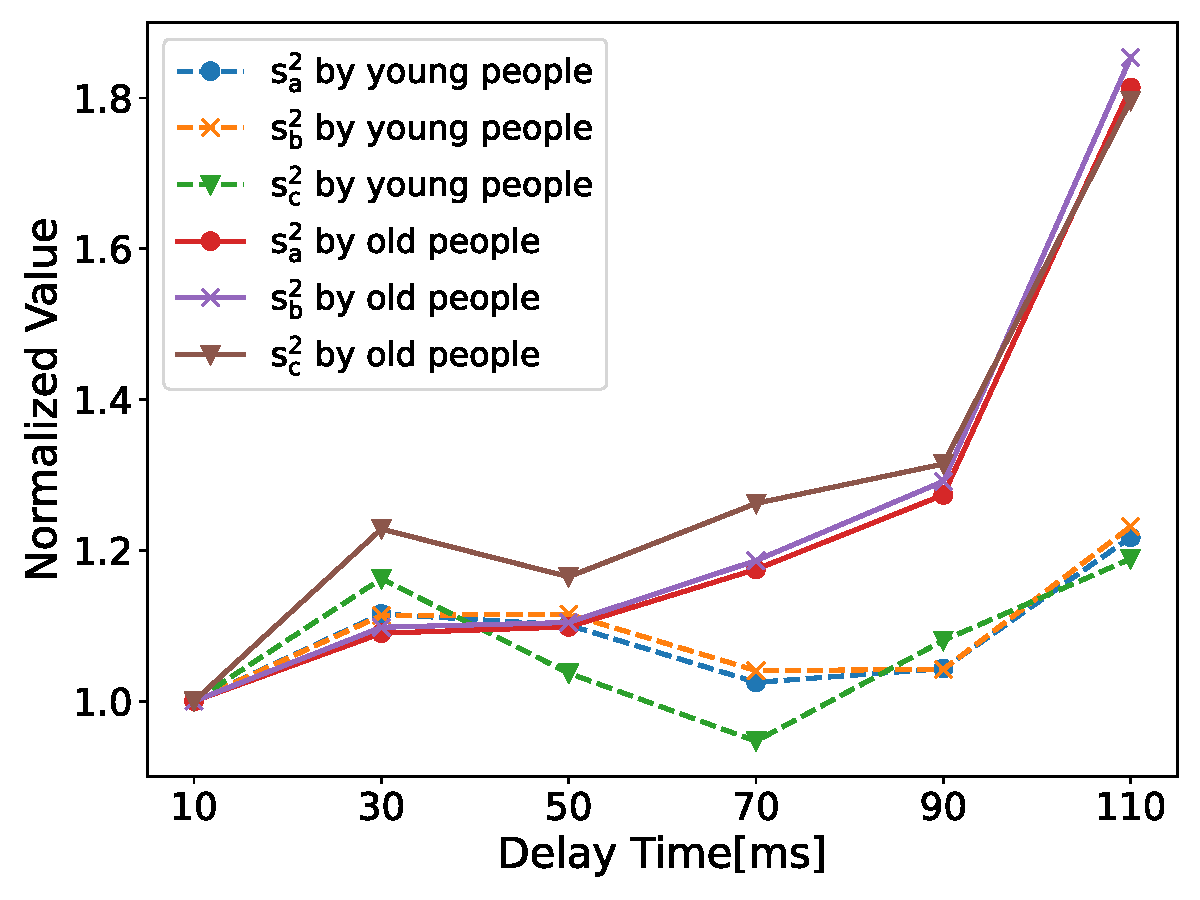
\includegraphics[scale=0.3]{figures/Honbann/Comparison_young_old/110_var_normalized.pdf}
  \caption{実験Aにおける若年者と高齢者の正規化後の評価値の比較}
  \label{fig:Normalized-Var_110ms_SaSbSc}
\end{figure}
\begin{figure}[tbp]
  \centering
  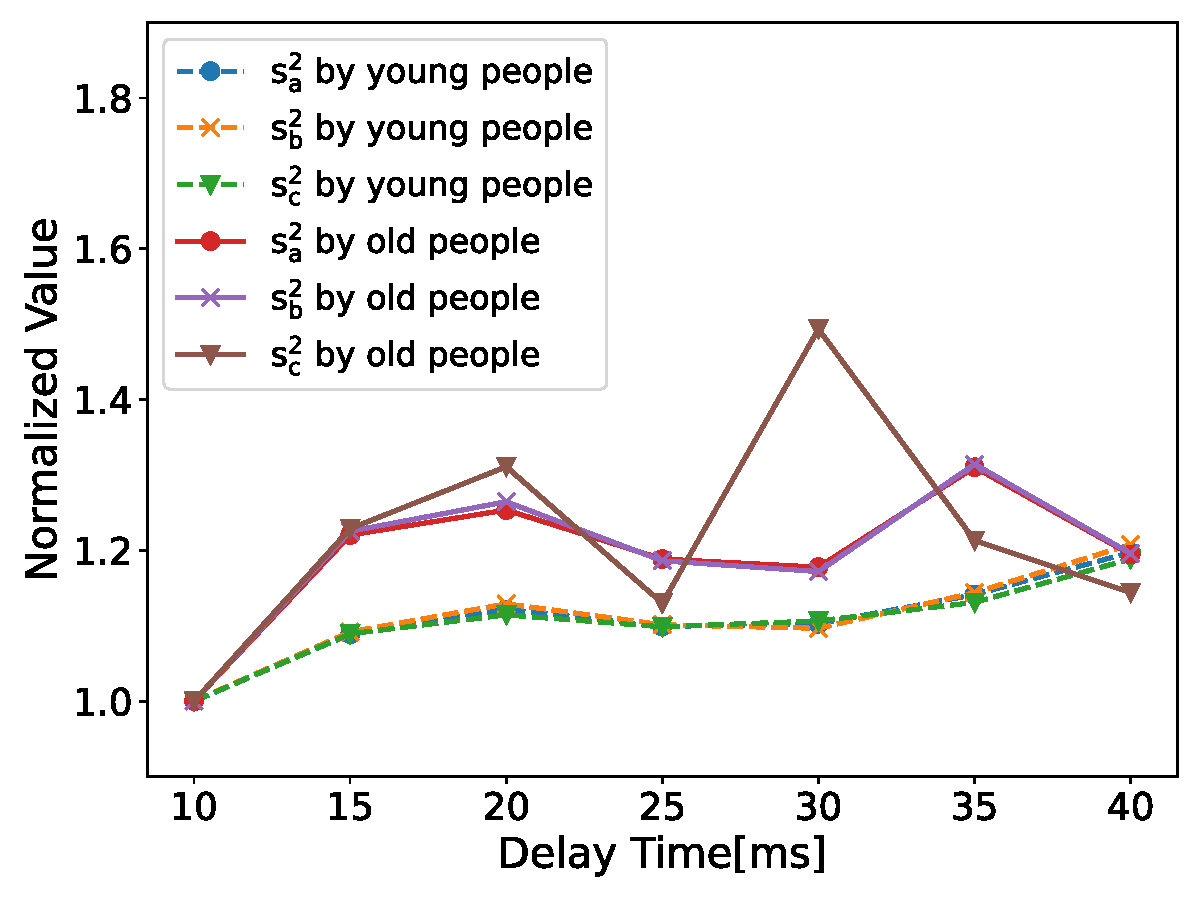
\includegraphics[scale=0.3]{figures/Honbann/Comparison_young_old/40_var_normalized.pdf}
  \caption{実験Bにおける若年者と高齢者の正規化後の評価値の比較}
  \label{fig:Normalized-Var_40ms_SaSbSc}
\end{figure}
\begin{figure}[tbp]
  \centering
  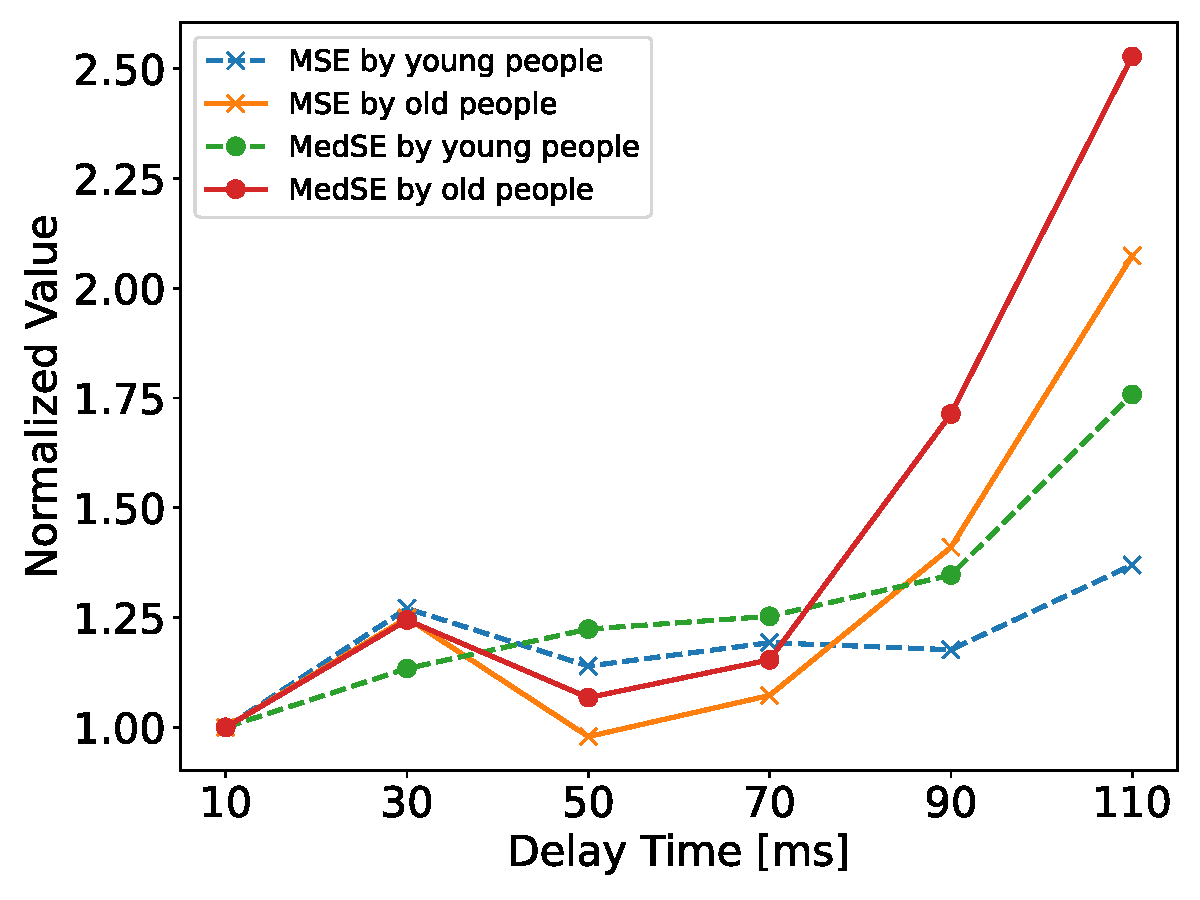
\includegraphics[scale=0.3]{figures/Honbann/Comparison_young_old/110_MSE-MedSE_normalized.pdf}
  \caption{実験Aにおける若年者と高齢者の正規化後のMSEとMedSEの比較}
  \label{fig:Normalized_110ms_MSE_MedSE}
\end{figure}
\begin{figure}[tbp]
  \centering
  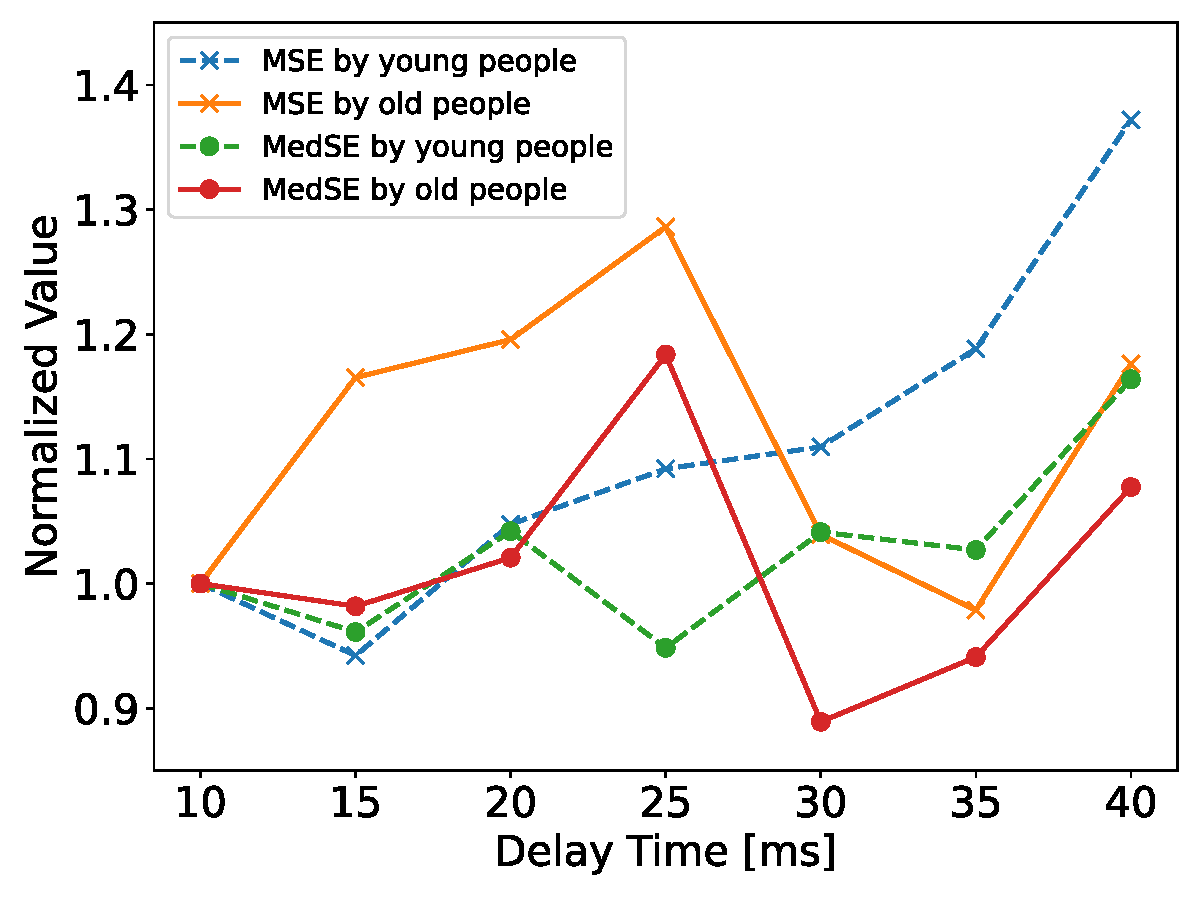
\includegraphics[scale=0.3]{figures/Honbann/Comparison_young_old/40_MSE-MedSE_normalized.pdf}
  \caption{実験Bにおける若年者と高齢者の正規化後のMSEとMedSEの比較}
  \label{fig:Normalized_40ms_MSE_MedSE}
\end{figure}